% vim: set tw=78 sts=2 sw=2 ts=8 aw et ai:

Having previously presented the various aspects that factor into MPTCP
performance, the current section describes how a highly configurable computer
network was modeled. A solution suitable to our analysis should preferably
yield similar results for several runs of a single test, grant the ability to
control the features outlined in Section \ref{sec:tcp-link} in a fine-grained manner
and also require comodity hardware. To this end, our experiments are based on
Mininet, a framework well suited for software defined networking. Being both
scalable and flexible, it conforms to the criteria mentioned above.

Mininet uses features of lightweight virtualization available on Linux
systems, such as process and network namespaces\cite{mininet}. There is a root
namespace, the default on a Linux system, which houses the switches, the
controller and the main management application. There is another distinct
namespace for each host, providing a network interface and a shell. The hosts'
interfaces are paired with counterparts in the root namespace and the shells
are piped to the management console, as can be observed in Figure
\ref{fig:mininet-design}. By using this approach, the overhead associated with
adding a new node to the simulation is negligible. Additionally, the framework
supports Open vSwitch, a virtual switch implemented in the kernel, for
modelling basic network equipment.

\begin{figure}
  \centering
  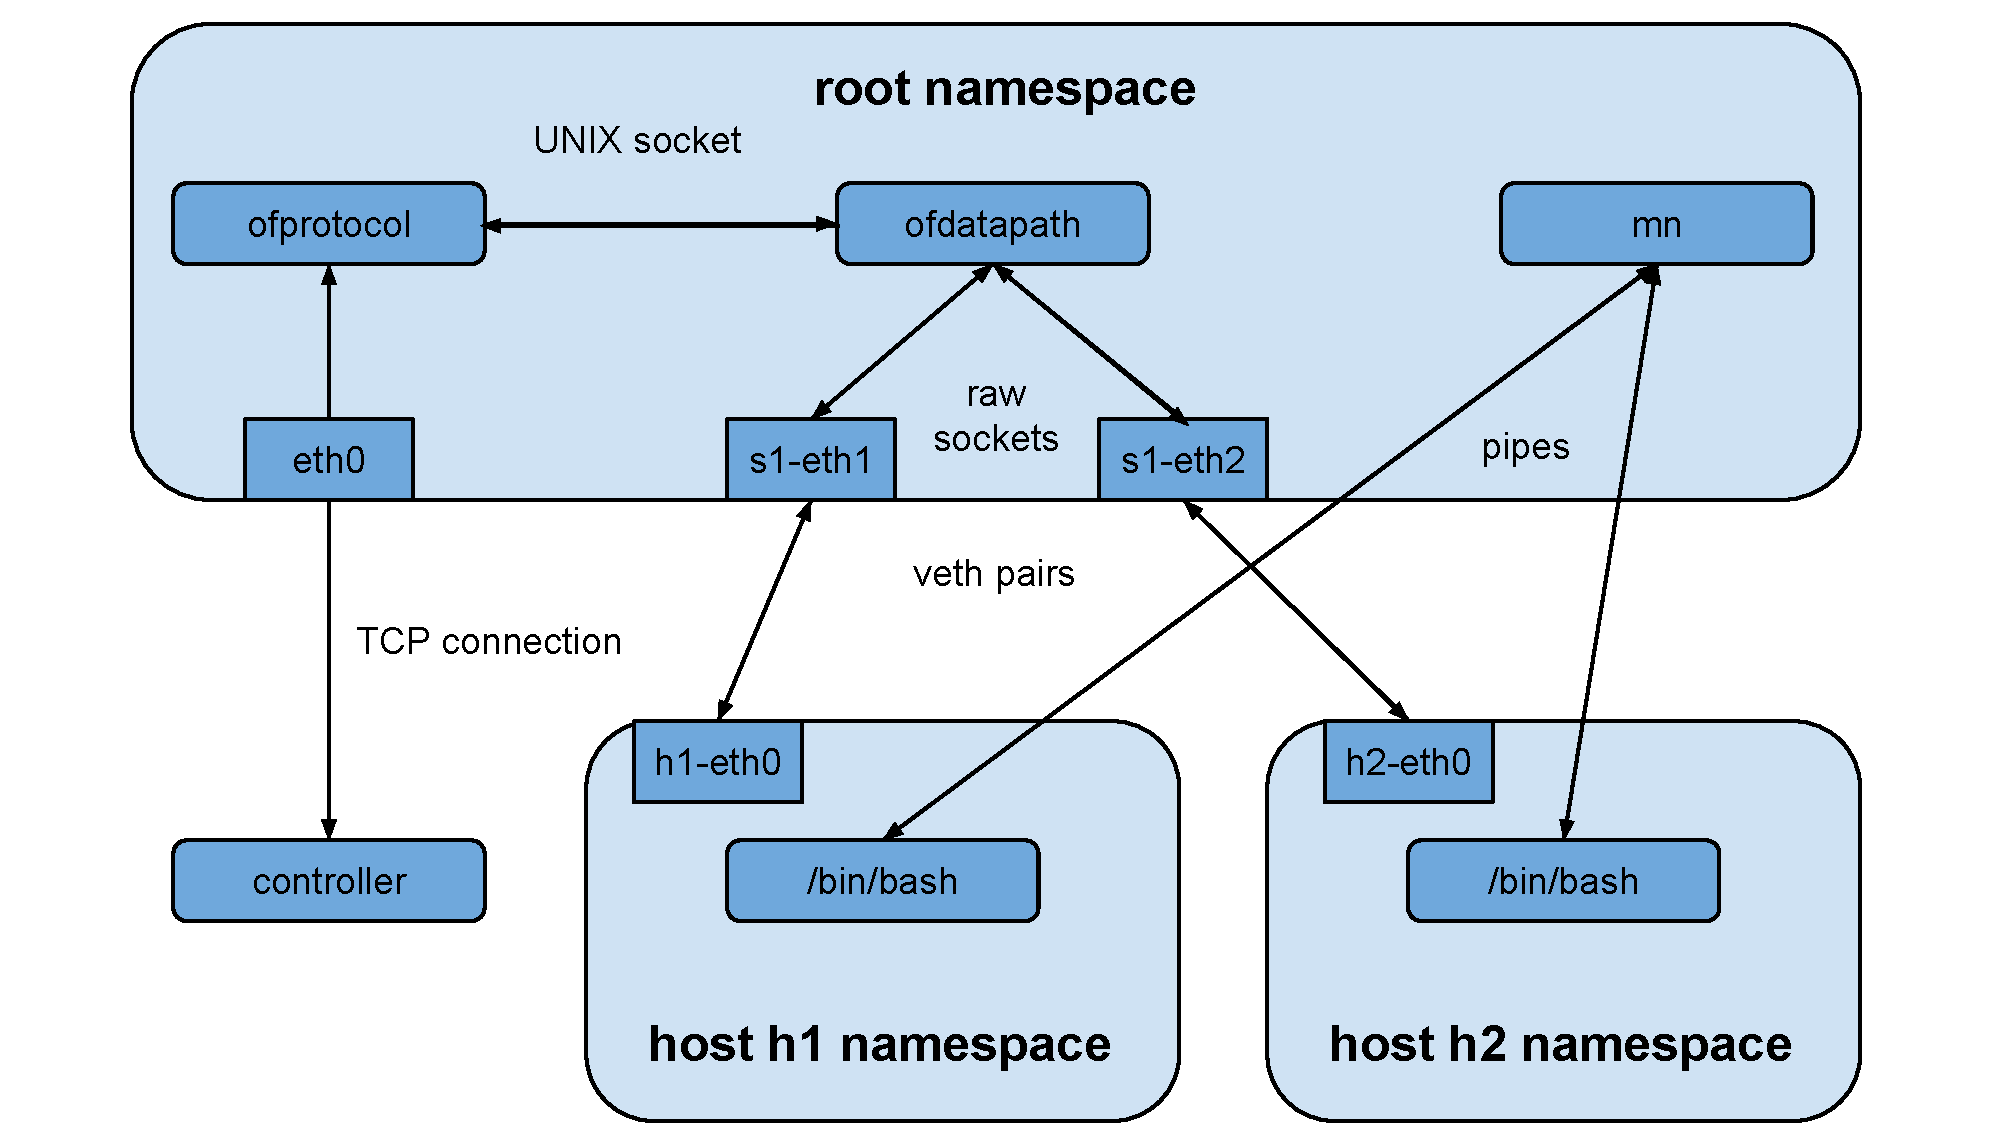
\includegraphics[width=0.85\textwidth]{img/mininet-design}
  \caption{Mininet namespaces}
  \label{fig:mininet-design}
\end{figure}

As far as flexibility goes, Mininet offers an elaborate prototyping
environment. Of all the characteristics described in \ref{sec:tcp-link},
only the TCP congestion window requires an external tool. All the other
parameters, which are Layer 2 specific, can be controlled using API calls.
Furthermore, since the API is targeted at Python, a high-level interpreted
language, topologies and simulations are easily developed.

In terms of validation of the Mininet framework as to whether it yields
relevant results or not, researchers have reproduced previous experiments
\cite{mininet-reproduce}. Not only were they able to recreate prior research
done with hardware testbeds, but thanks to the ease which Mininet simulations
can be reconfigured, they also managed to obtain extra results in some cases.

Considering the above-mentioned arguments, Mininet is undoubtedly an adequate
solution to model our tests. The testbed consists of a virtual machine running
Ubuntu 13.10 64-bit with a kernel supporting MPTCP and providing Mininet.
Using this setup, we define a simple topology using 2 hosts and 2 switches, as
seen in Figure \ref{fig:mininet-topo}. We then run iperf between the two hosts
while using different values for the link characteristics.

\begin{figure}
  \centering
  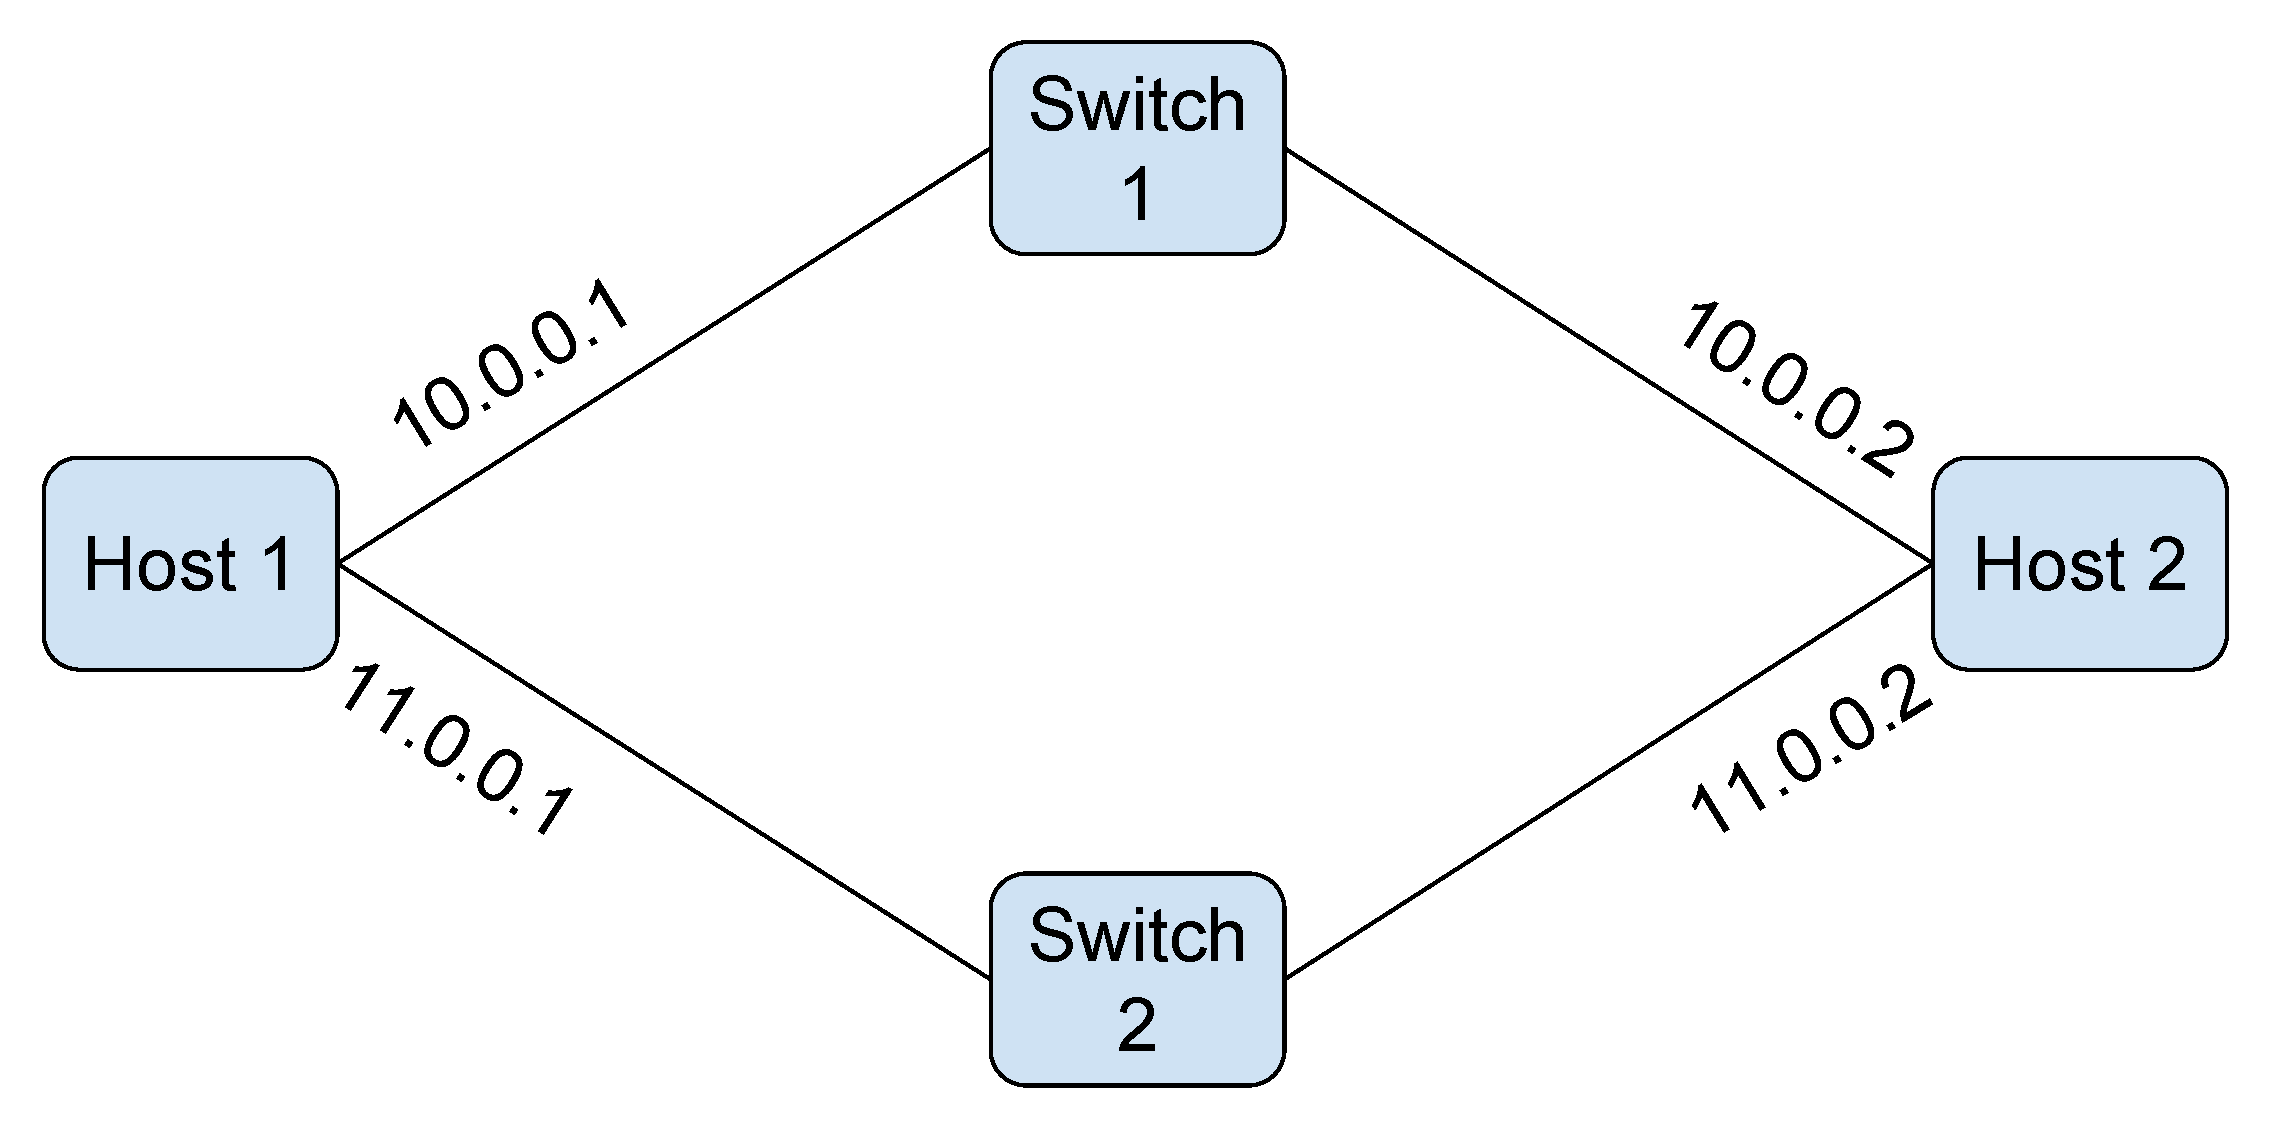
\includegraphics[width=0.7\textwidth]{img/mininet-topo}
  \caption{Mininet test topology}
  \label{fig:mininet-topo}
\end{figure}

